%!TEX root=../robocert.tex
\begin{figure}
	\centering
	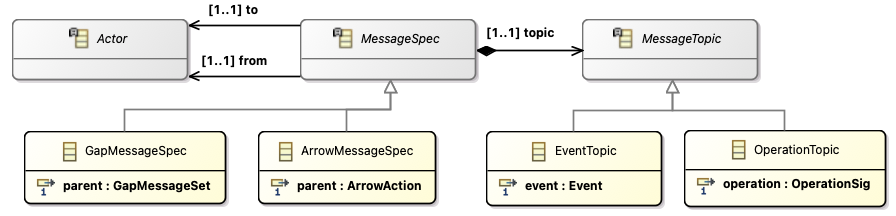
\includegraphics[width=\textwidth]{diagrams/messages.png}
	\caption{Class diagram for the part of the \langname{} metamodel dealing with messages.}
	\label{fig:metamodel-messages}
\end{figure}

\Cref{fig:metamodel-messages} depicts the part of the metamodel concerning
messages between actors.  Messages are introduced into a sequence diagram
in \mgapmessageset s and \marrowaction s.

\subsection{\mmessagespec}

A \mmessagespec{} is a specification on the types of communication that can
happen during a gap (a \mgapmessagespec) or arrow (an \marrowmessagespec).\footnote{
This class distinction resembles that in PSCs betweeen intraMSGs and arrowMSGs,
respectively.}  Each \mmessagespec{} contains:

\begin{itemize}
\item
	references to two \mactor s (\cref{sec:metamodel-actors}),
	capturing the source (\emph{from}) and destination (\emph{to})
	of the communication;
\item
	the \mmessagetopic{} (\cref{ssec:metamodel-messages-topics}) specifying
	the type of communication that the spec is capturing.
\end{itemize}

\begin{figure}[h]

\begin{subfigure}[t]{0.38\textwidth}
\begin{lstlisting}[style=Example]
operation O1() from M to W
// MessageSpec with OperationTopic

event E        from W to M
// MessageSpec with EventTopic
\end{lstlisting}
\end{subfigure}
\hfill
\begin{subfigure}[t]{0.58\textwidth}
\gsecaption
\centering
\begin{tikzpicture}
\matrix[diagram]{
    \node[rcmodule](mstart) {\egtarget}; & \node[world](wstart) {\egworld}; \\
	\coordinate(mo); & \coordinate(wo); \\
	\coordinate(me); & \coordinate(we); \\
	\coordinate(mend); & \coordinate(wend); \\
};
\draw[lifeline] (wstart) -- (wo) -- (we) -- (wend);
\draw[lifeline] (mstart) -- (mo) -- (me) -- (mend);
\draw (mo) edge[oarrow, "O1()"'] (wo);
\draw (we) edge[earrow, "E"] (me);
\end{tikzpicture}
\end{subfigure}

\end{figure}

\subsection{\mmessagetopic}\label{ssec:metamodel-messages-topics}

A \mmessagetopic{} identifies the specific type of communication in a
\mmessagespec{}.  There are currently two types of topic, corresponding to
\robochart{} operations (\moperationtopic) and events (\meventtopic).
Each contains a reference to the signature of the respective construct.
Parameterised operations and events are not yet supported \todo{this will
change}.

\begin{lstlisting}[style=Example]
operation O1() // OperationTopic
event E        // EventTopic
\end{lstlisting}

\subsection{\margument}\label{ssec:metamodel-messages-arguments}

A \margument{} is a pattern that specifies (and possibly binds) one or more
arguments in
a message.  There are two types of argument:

\begin{itemize}
\item
	\mexpressionargument, which specifies that the argument is equal to the
	value of a particular \robochart{} expression;
	\todo{the CSP generator doesn't yet properly protect against this being
	an expression not expressible as a prefix}
\item
	\mrestargument, which matches \emph{all} following arguments and permits
	them to be any value.
	\todo{This mainly exists because it's very easy to specify in CSP.  Ideally
	we'll have something that allows wildcards on arbitrary parameters, in
	which case this might be confusing to have also.}
\end{itemize}

All \margument s, at time of writing, are forms of \mnonbindingargument{} and
can therefore appear in \mgapmessagespec s.  This will change when binding
arguments are introduced.

\begin{lstlisting}[style=Example]
42  // ExpressionArgument containing integer literal
... // RestArgument
\end{lstlisting}
